
%%%%%%%%%%%%%%%%%%%%%%%%%%%%%%%%%%%%%%%%%%%%%%%%%%%%%%%%%%%%%%%%%%%%%%%%%%%%%%%%
%% BEFORE YOU START: 
%%
%% 1. Rename the paper.tex file into your paper name. Use the bibtex key policy 
%%    for the naming convention (see end of this file)
%%
%% 2. Change line 3 in the Makefile from "TARGET=paper" to "TARGET=name-of-tex-file"
%%
%%%%%%%%%%%%%%%%%%%%%%%%%%%%%%%%%%%%%%%%%%%%%%%%%%%%%%%%%%%%%%%%%%%%%%%%%%%%%%%%

\documentclass[letterpaper, 10 pt, conference]{ieeeconf}  % Comment this line out if you need a4paper
\IEEEoverridecommandlockouts                              % This command is only needed if
\overrideIEEEmargins                                      % Needed to meet printer requirements.

\usepackage{graphics}    % for pdf, bitmapped graphics files
\usepackage{times}       % assumes new font selection scheme installed
\usepackage{amsmath}     % assumes amsmath package installed
\usepackage{amssymb}     % assumes amsmath package installed
\usepackage{graphicx}
\usepackage{algorithm}
\usepackage[noend]{algpseudocode}

\usepackage{xcolor}

%% Align last page but causes error on some machines (such as OSX), so don't use for now.
%%\usepackage{flushend}

%% Style hacks to save space
%\setlength{\textfloatsep}{1.5em}
%\setlength{\dbltextfloatsep}{1.5em}
%\usepackage[font=small]{caption}

%% Key definitions for text elements. USE THEM
\def\secref#1{Sec.~\ref{#1}}
\def\figref#1{Fig.~\ref{#1}}
\def\tabref#1{Tab.~\ref{#1}}
\def\eqref#1{Eq.~(\ref{#1})}
\def\algref#1{Alg.~\ref{#1}}
\newcommand\etal{\emph{et al.}}

\usepackage{amsopn}


\newcommand{\bJidx}[1]{\ensuremath{\mathbf{J}^{[#1]}}}
\newcommand{\cose}{\mathrm{cose}}
\newcommand{\bzidx}[1]{\mathbf{z}^{[{#1}]}}
\newcommand{\bxidx}[1]{\mathbf{x}^{[{#1}]}}
\newcommand{\bhidx}[1]{\mathbf{h}^{[{#1}]}}
\newcommand{\bOmegaidx}[1]{\mathbf{\Omega}^{[{#1}]}}
\newcommand{\bSigmaidx}[1]{\mathbf{\Sigma}^{[{#1}]}}
\newcommand{\bHidx}[1]{\mathbf{H}^{[{#1}]}}

\newcommand{\bv}{\mathbf{v}}
\newcommand{\bl}{\mathbf{l}}
\newcommand{\bt}{\mathbf{t}}
\newcommand{\bo}{\mathbf{o}}
\newcommand{\bM}{\mathbf{M}}
\newcommand{\bL}{\mathbf{L}}
\newcommand{\bA}{\mathbf{A}}
\newcommand{\bB}{\mathbf{B}}
\newcommand{\bE}{\mathbf{E}}
\newcommand{\bK}{\mathbf{K}}
\newcommand{\bC}{\mathbf{C}}
\newcommand{\bG}{\mathbf{G}}
\newcommand{\bH}{\mathbf{H}}
\newcommand{\bI}{\mathbf{I}}
\newcommand{\bP}{\mathbf{P}}
\newcommand{\bX}{\mathbf{X}}
\newcommand{\bZ}{\mathbf{Z}}
\newcommand{\bR}{\mathbf{R}}
\newcommand{\bS}{\mathbf{S}}
\newcommand{\bU}{\mathbf{U}}
\newcommand{\bV}{\mathbf{V}}
\newcommand{\bT}{\mathbf{T}}
\newcommand{\bpi}{\mathbf{\pi}}
\newcommand{\btl}{\mathbf{tl}}
\newcommand{\bbr}{\mathbf{br}}


\newcommand{\iD}{\mathbf{D}}
\newcommand{\iN}{\mathbf{N}}
\newcommand{\iI}{\mathbf{I}}

\newcommand\norm[1]{\left\lVert#1\right\rVert}

\newcommand{\bzridx}[1]{\ensuremath{\mathbf{z}^{({#1})}}}
\newcommand{\bxridx}[1]{\mathbf{x}^{({#1})}}
\newcommand{\bhridx}[1]{\mathbf{h}^{({#1})}}

\newcommand{\bJ}{\mathbf{J}}
\newcommand{\bZero}{\mathbf{0}}

\newcommand{\cS}{\mathcal{S}}
\newcommand{\cG}{\mathcal{G}}
\newcommand{\cE}{\mathcal{E}}
\newcommand{\cC}{\mathcal{C}}
\newcommand{\cSM}{\mathcal{SM}}
\newcommand{\cR}{\mathcal{R}}
\newcommand{\cM}{\mathcal{M}}
\newcommand{\cP}{\mathcal{P}}
\newcommand{\cL}{\mathcal{L}}
\newcommand{\cD}{\mathcal{D}}
\newcommand{\cZ}{\mathcal{Z}}
\newcommand{\cX}{\mathcal{X}}
\newcommand{\range}[3]{#1_{#2:#3}}


\newcommand{\ba}{\mathbf{a}}
\newcommand{\bb}{\mathbf{b}}
\newcommand{\bc}{\mathbf{c}}
\newcommand{\bd}{\mathbf{d}}
\newcommand{\be}{\mathbf{e}}
\newcommand{\ec}{\mathbf{e}}
\newcommand{\bm}{\mathbf{m}}
\newcommand{\bg}{\mathbf{g}}
\newcommand{\Dim}{\mathrm{Dim}}

\newcommand{\bs}{\mathbf{s}}
\newcommand{\bx}{\mathbf{x}}
\newcommand{\by}{\mathbf{y}}
\newcommand{\br}{\mathbf{r}}
\newcommand{\bz}{\mathbf{z}}
\newcommand{\bu}{\mathbf{u}}
\newcommand{\bn}{\mathbf{n}}
\newcommand{\bh}{\mathbf{h}}
\newcommand{\bff}{\mathbf{f}}
\newcommand{\bp}{\mathbf{p}}
\newcommand{\bDelta}{\mathbf{\Delta}}
\newcommand{\bGamma}{\mathbf{\Gamma}}
\newcommand{\bDeltaalpha}{\mathbf{\Delta \alpha}}
\newcommand{\bDeltar}{\mathbf{\Delta r}}
\newcommand{\bDeltax}{\mathbf{\Delta x}}
\newcommand{\bDeltaX}{\mathbf{\Delta X}}
\newcommand{\bDeltat}{\mathbf{\Delta t}}
\newcommand{\bDeltaR}{\mathbf{\Delta R}}
\newcommand{\tTov}{\mathrm{t2v}}
\newcommand{\vTot}{\mathrm{v2t}}

\newcommand{\bO}{\mathbf{O}}

\newcommand{\defeq}{=}


\newcommand{\bmu}{\mathbf{\mu}}
\newcommand{\bnu}{\mathbf{\nu}}
\newcommand{\bSigma}{\mathbf{\Sigma}}
\newcommand{\bOmega}{\mathbf{\Omega}}
\newcommand{\bLambda}{\mathbf{\Lambda}}

\newcommand{\mat}[1]{#1}
\newcommand{\mbf}[1]{\mathbf{#1}}
\newcommand{\defn}[1]{\emph{#1}}

\newcommand{\mysum}{\sum}
\newcommand{\myprod}{\prod}
\newcommand{\eq}{=}
\newcommand{\pv}{\mathrm{P}}
%\newcommand{\implies}{\Rightarrow}
\newcommand{\Parents}{\mathrm{Parents}}
\newcommand{\rj}{\mathrm{j}}
\newcommand{\proj}{\mathrm{proj}}
\DeclareMathOperator*{\argmax}{argmax}
\DeclareMathOperator*{\argmin}{argmin}
\DeclareMathOperator*{\atantwo}{atantwo}

\newcommand{\mR}{\mathbb{R}}
\newcommand{\mN}{\mathbb{N}}
\newcommand{\mC}{\mathbb{C}}



%% Other useful macros
\newcommand\todo[1]{\textbf{[TODO: #1}]}

%% Some math definition
\def\argmax{\mathop{\rm argmax}}
\def\argmin{\mathop{\rm argmin}}
\newcommand{\bigO}[1]{$\mathcal{O}(#1)$}


%%%%%%%%%%%%%%%%%%%%%%%%%%%%%%%%%%%%%%%%%%%%%%%%%%%%%%%%%%%%%%%%%%%%%%%%%%%%%%%%
\title{\LARGE \bf Active Semantic Mapping}

\author{Federico Nardi \and Roberto Capobianco \and Daniele Nardi% <-this % stops a space
	\thanks{All authors are with the Sapienza University of Rome, 
		Department of Computer, Control, and Management Engineering  "Antonio Ruberti", Rome, Italy. }%
	%\thanks{This work has partly been supported by ...
	%the EC under the grant number H2020-ICT-644227-Flourish. 
	%the EC under the grant number H2020-ICT-645403-RobDREAM.
	%the DFG under the grant number FOR~1505: Mapping on Demand.
	%}%
}

\begin{document}
\maketitle
\thispagestyle{empty}
\pagestyle{empty}


%%%%%%%%%%%%%%%%%%%%%%%%%%%%%%%%%%%%%%%%%%%%%%%%%%%%%%%%%%%%%%%%%%%%%%%%%%%%%%%%
\begin{abstract}
  %
  % WHY is it relevant
  \emph{1-2 not too long sentences clearly answering the WHY question.}
  
  % WHICH PROBLEM are we adressing
  In this paper, we present a ....  . 

  % HOW is our approach special, WHAT are we actually doing, and WHAT IS NEW
  Our approach ... \emph{(complete, around 2-3 sentences)}
 
  %% IMPLEMENTATION, EVALUATION, WHAT FOLLOWS 
  We implemented our approach using C++ and ROS and thoroughly tested
  it on .... \emph{(finish sentence)}. The experiments presented in
  this paper show that ... \emph{(finish sentence)}
\end{abstract}


%%%%%%%%%%%%%%%%%%%%%%%%%%%%%%%%%%%%%%%%%%%%%%%%%%%%%%%%%%%%%%%%%%%%%%%%%%%%%%%%
\section{Introduction}
\label{sec:intro}

%% WHY 
{\color{blue}\emph{WHY: First, answer the WHY question. You MAY but do not have to
  briefly refer to a small number of other works.}}

\paragraph{Sometimes active perception is needed} the last decade has seen tremendous advances in building accurate digital models of the robot workspace. State-of-the-art reconstruction and recognition approaches enable the robot to store precise geometric and semantic information of objects/places in its internal representation of the environment.

Still, some tasks require the robot to acquire a rich amount of information about its workspace. As an example, for object manipulation the robot needs to know the position of the objects in the scene and their shape to plan a motion trajectory.

To represent this information a possible solution is to use CAD models. While effective, this approach has the limitation that the perceivable objects must be known a priori. To overcome this limitation, one must provide the robot with the ability of actively building such models to support task execution.

	

%% WHICH PROBLEM
{\color{blue}\emph{WHICH PROBLEM: Second, explain WHICH problem you are solving. You MAY briefly 
 refer to 1-2 other works or standard approaches and what you do differently.}}

\paragraph{building a usable representation} we are solving the problem of building a digital representation of the robot workspace that can support task execution.

%% HOW & WHAT; already briefly mention what is novel (but go more in detail in the next paragraph)
{\color{blue}\emph{HOW: Third, explain briefly HOW your approach is special and then WHAT 
you do concretely.} }

\paragraph{enrich semantic mapping with active perception} To this end, we enrich the robot software architecture with an active vision module.

\paragraph{active semantic mapping} the active vision strategy takes as input the semantic map and returns the NBV that increases the robot knowledge about a particular object.

\begin{figure}[t]
  \centering
 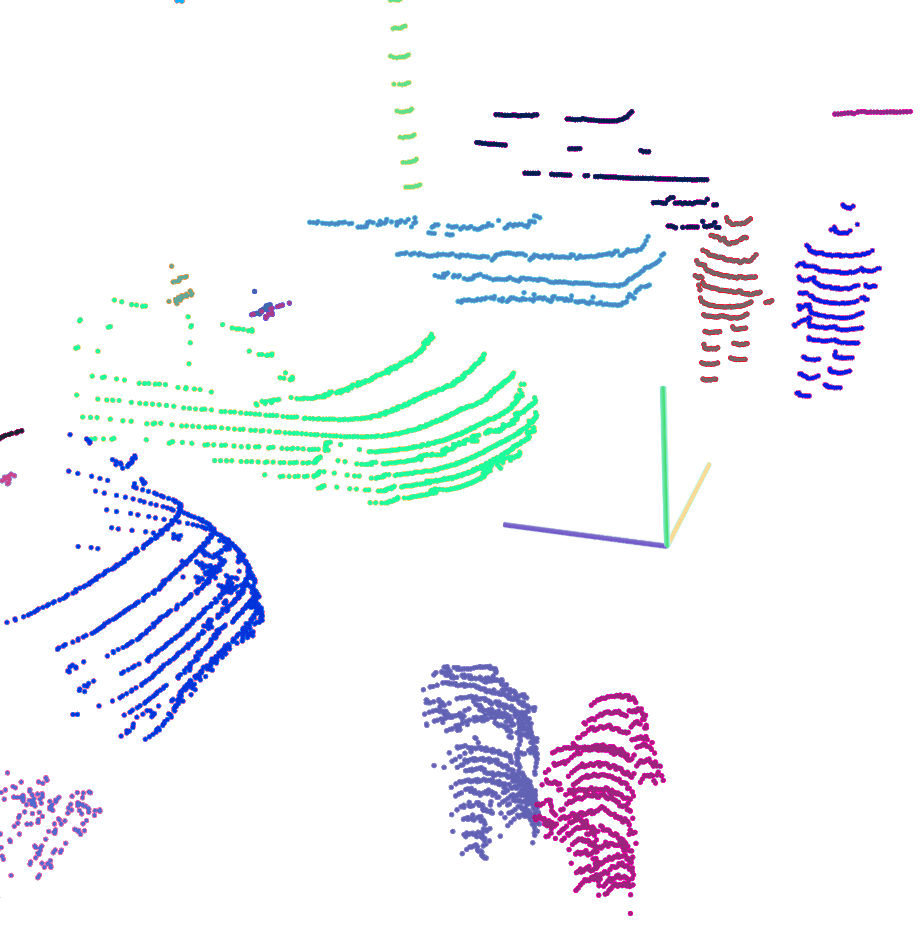
\includegraphics[width=0.99\linewidth]{pics/motivation}
 \caption{Motivating Example. Providqe a caption that lets the reader
   understand the image easily.  This image should be on top of the
   right column of page~1.}
  \label{fig:motivation}
\end{figure}

%% MAIN CONTRIBUTION & WHAT FOLLOWS FROM THAT
\emph{Explain your contribution in one paragraph. Start that paragraph with:}

The main contribution of this paper is a ....  We achieve this by
... This allows us to ... See \figref{fig:motivation} for an example.

%% CLAIMS (can be merged with main contribution)
\emph{Claims: Explicitly state your claims in one paragraph using (i)
  ..., (ii) ..., (iii) ... and, if useful, spell out the key
  assumptions. You can do that here or merge the caims with the
  previous paragraph about the main contribution. For example:}

In sum, we make N key claims, which are are the follwing:
Our approach is able to
%
(i) ..., 
%
(ii) ..., 
%
(iii) ... and,
%
(iv) . 
% 
These N claims are backed up by the paper and especially 
our experimental evaluation.


%%%%%%%%%%%%%%%%%%%%%%%%%%%%%%%%%%%%%%%%%%%%%%%%%%%%%%%%%%%%%%%%%%%%%%%%%%%%%%%%
\section{Related Work}
\label{sec:related}

%\emph{Discuss the main related work and cite around 12-20 papers in
%  sum. The related work section should be approx. 1 column long
%  assuming a 6-page paper. Structure the section in paragraphs,
%  grouping the papers, and describing the key approaches with 1-2
%  sentences. If applicable, describe the key difference to your
%  approach at the end of each paragraph briefly. Avoid adding
%  subsections for a conference paper.}
%
%\emph{Example text fragments: }
%
%The approach by Neubert \emph{et al.}~\cite{neubert13ecmr} aims at
%predicting ...
%
%Biber and Duckett~\cite{biber05rss} address the problem of dealing
%with...
%
%In contrast to that, Stachniss and Burgard~\cite{stachniss05aaai}
%model different instances of typical world states using clustering.
%
%There are furthermore approaches that combine ....  at city
%scale~\cite{churchill13ijrr}.
%
%\emph{If useful, BIEFLY summarize your key contributions again at the
%  end, for example:} In this paper, we introduce a ... scheme that is
%inspired by the work of H\"ahnel \emph{et al.}~\cite{haehnel03isrr}
%but it extends the original ideas by ...

The problem of building a \emph{usable} representation of the environment is addressed by facing three aspects: 1) processing sensor data to extract geometric and semantic information, 2) modeling these information in a suitable representation that support task execution and 3) planning the robot motion to maximize the extraction of such information.

\subsection{Perception}

\subsection{Map Construction}

\subsection{Exploration}

%%%%%%%%%%%%%%%%%%%%%%%%%%%%%%%%%%%%%%%%%%%%%%%%%%%%%%%%%%%%%%%%%%%%%%%%%%%%%%%%
\section{Our Approach}
\label{sec:main}

%\emph{Describe your approach. It is okay to divide the main section
%  into a few subsection (e.g., 2-4 subsections).}
%
%
%Use equations in the style of
%\begin{eqnarray}
%\label{eq:nameeqn}
%  p(x) &=& \alpha + \beta.
%\end{eqnarray}
%
%In \eqref{eq:nameeqn}, the term~$\alpha$ refers to ...
%
%\emph{A few comments:
%\begin{itemize}
%	\item Add a tilde (\textasciitilde) in front of inline math (using \$) to avoid a line break.
%	\item Add a tilde (\textasciitilde) in front of a cite to avoid a line break.
%	\item Use the macros \textbackslash{}figref, \textbackslash{}tabref, \textbackslash{}secref, \textbackslash{}eqref for referencing
%	\item Separate number and units using \textbackslash{}, for example 1\textbackslash{},m, which results in 1\,m
% \end{itemize}
%}

A semantic map is a collection of elements

\begin{equation}
\cSM = \{ \bE_1 \dots \bE_N \},
\end{equation}

where each element $\bE_i = < \cG_i, \cS_i>$ represents an object in the scene and is characterized by geometric and semantic information.

\subsection{Geometric Information $\cG$}

The former describes the geometric properties of each element of the map. To fully qualify an element geometry we make us of:
\begin{itemize}
	\item {\bf Pose3D}: $\bX = [ \bR | \bt] \in SE(3)$, it's expressed in a global reference system $\cR^G$ and defines the element reference system $\cR^E$.
	\item {\bf Size3D}: $\bS = <\bL ,\bU> \in \mathbf{R}^3 $, it's represented by two 3D vectors that define the smallest \emph{axis-aligned} bounding box that contains the whole element.
	\item {\bf Representation3D}: $\bM$, a digital model of the element surface (e.g. point cloud, mesh and so on).
\end{itemize}

\subsection{Semantic Information $\cS$}

While, the latter describes the semantic information of each elements of the map through the following properties:
\begin{itemize}
	\item {\bf Type}: $t \in \cL$, the element category. It's selected by the recognition module among the possible semantic labels $\cL = \{l_1 \dots l_M \}$.
	\item {\bf Properties:} $\bP = \{ p_1 \dots p_K \}$, other semantic information related to the element, e.g. relationships with other elements, physical properties, functionalities, and so on. 
\end{itemize}   

\subsection{Semantic Mapping Process}

To build such a representation, the semantic mapping process can be decomposed in three steps (see~\figref{fig:system}): \emph{1) perception}, the output of visual and range sensors is processed to extract information for recovering the structure and objects/places categories of the scene; \emph{2) map management}, these information is used to update the current belief about the state of the environment; \emph{3) action}, next pose for the robot is computed in order to improve its representation of the environment. In the remainder, we will present a detailed description of each of these sub-problems along with our proposed implementation.



%%%%%%%%%%%%%%%%%%%%%%%%%%%%%%%%%%%%%%%%%%%%%%%%%%%%%%%%%%%%%%%%%%%%%%%%%%%%%%%%
\section{Experimental Evaluation}
\label{sec:exp}

\emph{Repeat the main focus/objective with one sentence starting with:}
%
The main focus of this work is a  ..... 

\emph{Explain the reader that the experiments with support all claims
  (same list as in the intro!) starting the paragraph with:} 
%
Our experiments are designed to show the capabilities of our method and to
support our key claims, which are: 
%
(i)~..., 
%
(ii)~..., 
%
(iii)~..., and
%
(iv)~....

We furthermore provide comparisons to a popular method for ... as
proposed in~\cite{}.  We perform the evaluations on own datasets as
well as on publicly available ones.  Throughout all these experiments,
we set the key parameter of our approach to $X=1$ as this provided the
best performance as shown in \figref{fig:parameval}.

\emph{If needed (and only then!) say also a few words about the
  experimental setup, the datasets, and used parameters. You can use
  an own subsection if you want to put focus on that but often that is
  not needed.}

\emph{Note 1: It MUST be always crystal clear (a) WHY an experiment is
  there (e.g., to support a claim, to show that the approachis useful
  for real word systems, to show the performance, or to provide a
  baseline comparison), (b) WHAT it wants to show (which
  claim/property exactly), and (c) HOW it aims at showing this. This
  is ESSENTAIL for a good evaluation. Think about when BEFORE
  designing an experiment.}

\emph{Note 2: Start with the most important/impressive experiment
  first. Make this a key story of the paper. Keep the order of the
  claims, i.e., re-order claims in the intro/before if needed. }

%%%%%%%%%%%%%%%%%%%%%%%%
\subsection{Performance}

\emph{Start EVERY experiment with a similar start as the following
  sentence, explaining in the first sentence why you present the
  experiment and which claim it aims at supporting.}

%% First experiment - most impressive, important or the most important
%% claim supporting experments comes first.
The first experiment is designed to show the performance of our
approach and to support the claim that it is well-suited for ....

\begin{figure}[t]
  \centering
 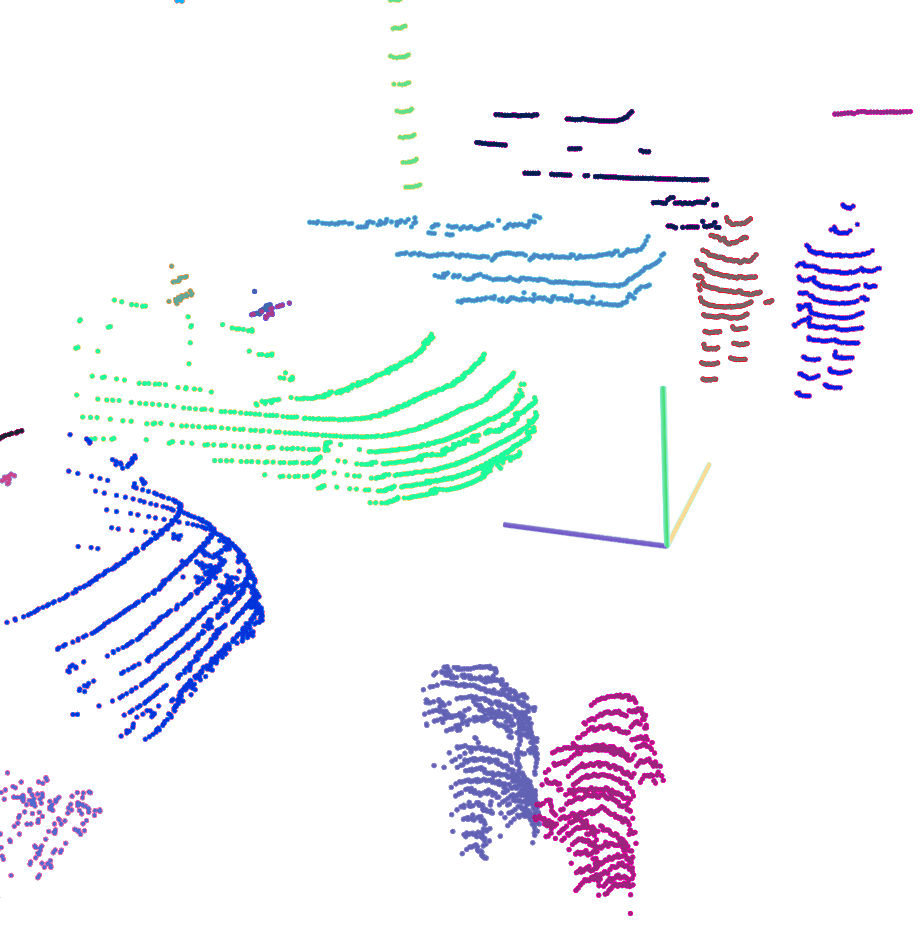
\includegraphics[width=0.99\columnwidth]{pics/motivation}
  \caption{A caption that makes you understand the image easily.}
  \label{fig:parameval}
\end{figure}

%% Second experiment - could be a comparison to a baseline methods,
%% quality analysis or similar
The second experiment is to support the claim that our approach is ...

%%%%%%%%%%%%%%%%%%%%%%%%
\subsection{Runtime}

%% Rumtime experiment - it is often one of the last experimemts unless
%% online processing / speed is the key contribution
The next set of experiments in designed to support the claim that our
approach runs fast enough to support online processing on the robot in
real time. We therefore tested our approach on ....

\tabref{tab:speed} summarizes the runtime results for .....  The
numbers support our third (check!) claim, namely that the computations
can be executed fast and in an online fashion.  On a mobile i5 CPU, we
achieve average frame rates of XXX\,Hz-XXX\,Hz depending on ... and
XXX\,Hz-XXX\,Hz on an i7 desktop computer.
 
\begin{table}
\caption{Average runtime and std.~dev.}
\centering
{\footnotesize
\begin{tabular}{|c|c|c|}
\hline
XXXX & mobile & desktop \\
 & i5 CPU 2.2\,GHz & i7 CPU 3.5 GHz\\
\hline
configA & 2.4\,ms~$\pm$~0.5\,ms~$\approx$~416\,Hz & 1.5\,ms~$\pm$~0.2\,ms~$\approx$~667\,Hz \\
configB & 4.4\,ms~$\pm$~1.2\,ms~$\approx$~227\,Hz & 2.6\,ms~$\pm$~0.5\,ms~$\approx$~385\,Hz \\
configC & 8.6\,ms~$\pm$~2.6\,ms~$\approx$~116\,Hz & 4.7\,ms~$\pm$~1.2\,ms~$\approx$~212\,Hz \\
\hline
\end{tabular}
}
\label{tab:speed}
\end{table}

%%%%%%%%%%%%%%%%%%%%%%%%
\subsection{XXX Analysis}

Finally, we aim at supporting our claim that ....

\emph{Briefly summarize the evaluation and what follows with approx. 2
  sentences.}  In summary, our evaluation suggests that our method
provides competitive .... At the same time, our method is fast enough
for online processing and has small memory demands. Thus, we supported
all our claims with this experimental evaluation.


%%%%%%%%%%%%%%%%%%%%%%%%%%%%%%%%%%%%%%%%%%%%%%%%%%%%%%%%%%%%%%%%%%%%%%%%%%%%%%%%
\section{Conclusion}
\label{sec:conclusion}

In this paper, we presented novel approach to.....  
Our approach operates ....  Our method exploits ....  
This allows us to successfully ...  
We implemented and evaluated our approach on different datasets
and provided comparisons to other existing techniques and supported
all claims made in this paper. The experiments suggest that ...


%%%%%%%%%%%%%%%%%%%%%%%%%%%%%%%%%%%%%%%%%%%%%%%%%%%%%%%%%%%%%%%%%%%%%%%%%%%%%%%%
% Future work only if it makes sense 
\emph{Future work: Use only if applicable -- but if so, use the
  following sentence to start:} 

Despite these encouraging results, there is further space for
improvements. For example, ...


%%%%%%%%%%%%%%%%%%%%%%%%%%%%%%%%%%%%%%%%%%%%%%%%%%%%%%%%%%%%%%%%%%%%%%%%%%%%%%%%
% Only if applicable
%\section*{Acknowledgments}
%We thank XXX for fruitful discussions and for ...

\bibliographystyle{plain}
\bibliography{robots}

\end{document}

%%%%%%%%%%%%%%%%%%%%%%%%%%%%%%%%%%%%%%%%%%%%%%%%%%%%%%%%%%%%%%%%%%%%%%%%%%%%%%%%
%% NOTES ON PAPER WRITING
%
% Rename the paper.tex file into your paper name. Use the bibtex key policy (see below)
%
% Use a Spell Checker with US English as spelling language
% 
% Use Academic Writing Check: https://github.com/devd/Academic-Writing-Check
%
% Use GIT for version control. Use our gitlab sever!
%
% Make sure your Makefile is working correctly and compiles the documents 
%
% All images go to the subfolder pics and reviews into the revoiews folder
%
% Make sure the source files for images are in the pics folder as well (unless they are huge)
%
%%%%%%%%%%%%%%%%%%%%%%%%%%%%%%%%%%%%%%%%%%%%%%%%%%%%%%%%%%%%%%%%%%%%%%%%%%%%%%%%


%%%%%%%%%%%%%%%%%%%%%%%%%%%%%%%%%%%%%%%%%%%%%%%%%%%%%%%%%%%%%%%%%%%%%%%%%%%%%%%%
%% NOTES ON BIB ENTRIES
%
% Bibtex Key Policy
%
%    All in lower case
%    Use the key structure: <lastnamefirstauthor><2 digit year><conference/journal><extra>
%    Use <extra>:
%        for workshops: -ws,
%        for multiple papers: -a, -b, -c, ... ordered by title in alphabetical order
%        additionally add -a, -b, -c, ... ordered by title in alphabetical order in case of multiple workshops
%    Examples: stachniss08icra, stachniss08icra-ws, stachniss08icra-a, stachniss08icra-b
%    Use the bibtex key also at the filename for the paper, e.g., stachniss08icra.pdf
%
% Bibtex Entries
%
%    Use strings for conferences and journal name in order to keep obtain consistent entries
%    Use the identical abbreviations for conference name, e.g., “Proc. of the IEEE Int. Conf. on Robotics and Automation (ICRA)”
%    Avoid adding location in addition to the city or street of the conference.
%    Use doi for the official document on the publisher webpage. 
%    Abbreviate the first name of the authors, e.g., C. Stachniss instead of Cyrill Stachniss
%    In case of a first name and a middel name, use no space between them, e.g., C.J. Stachniss
%%%%%%%%%%%%%%%%%%%%%%%%%%%%%%%%%%%%%%%%%%%%%%%%%%%%%%%%%%%%%%%%%%%%%%%%%%%%%%%%


